\section{\lqpl{} statements}\label{sec:lqplstatements}
The \lqpl{} language has  the following statements:
\begin{description}
\item{\emph{Assignment}:} The assign statement, e.g. \inlqpl{x=t};
\item{\emph{Classical control}:} The
\inlqpl{if} - \inlqpl{else} statement.
\item{\emph{Case}:} The \inlqpl{case} for operating on constructed
data types.
\item{\emph{Measure}:} The \inlqpl{measure} statement which measures
a \qbit{} and executes dependent statements.
\item{\emph{Use}:} The
\inlqpl{use} and classical assign statements which operate on classical
data, moving it on to the classical stack for processing.
\item{\emph{Function calls}:} The various ways of calling functions or applying
transformations.
\item{\emph{Blocks}:} A group
of statements enclosed by '\{' and '\}'.
\item{\emph{Quantum control}:} Control of statements by 
 the \inlqpl{<=} qualifier.
\item{\emph{Divergence}:} The \inlqpl{zero} statement.
\item{\emph{Other}:} the \inlqpl{discard} statement.
\end{description}
\subsection{Assignment statement}\label{subsec:assignmentstatement}
Assignments create variables. Typical
examples of these are:
\begin{lstlisting}
        q1 = |0>;
        i = 42;
        bt1 = Br(Leaf (q1), Br (Leaf(|0>),Leaf(|1>)));
\end{lstlisting}
Here the first line creates a \qbit{}, \inlqpl{q1}, 
with initial value \ket{0}. The
second line creates an integer ,\inlqpl{i},
  with the value $42$. The last line creates a
binary tree, \inlqpl{bt1},
 with \inlqpl{q1} as its leftmost node, and the right node
being a sub-tree with values \ket{0} and \ket{1} in the left and 
right nodes respectively. Note that after the execution of the 
third statement, the variable \inlqpl{q1} is no longer in scope so the
name may be reused by  reassigning some other value to it.

The variables  on the left hand side of an
assignment are always quantum variables.
\paragraph{Syntax of assignment statements.} An assignment statement always
begins with an \emph{identifier}. This
must be followed by a single equals sign and then an \emph{expression}.

Identifiers in \lqpl{} must always start with a lower case letter.

Expressions are discussed below in \vref{sec:lqplexpressions}

\subsection{Classical control}\label{subsec:classicalcontrolstatements}
Classical control provides a way to choose sets of instructions
to execute based upon the values on the classical stack. 

\begin{figure*}[htbp]
\begin{singlespace}
\lstinputlisting[style=linqpl]{examplecode/lowprime.qpl}
\end{singlespace}
\caption{\lqpl{} program demonstrating \inlqpl{if-else}}
\label{fig:defsec:stmts:demoofifelse}
\end{figure*}

The expressions in the selectors 
\emph{must} be classical. This means they can only consist of
operations on  constants and classical identifiers. 
It is a semantic error to 
have an expression that depends on a
quantum variable. For an example, see the code to determine if
an input number is a small prime in \vref{fig:defsec:stmts:demoofifelse}.

\paragraph{Syntax of the \inlqpl{if -} \inlqpl{else} statement.} 
The statement starts
with the word \emph{if}, followed by one or more \emph{selectors}.
Each selector is composed of a classical Boolean expression $e_b$, the
symbols \emph{=>} and a dependent block. 
 The statement is 
completed by a special selector where the Boolean expression is
replaced with the word \emph{else}. 

In the list of $e_i => b_i$ selectors, 
$b_i$ is executed only when $e_i$ is the first expression to
evaluate to \inlqpl{true}. All others are skipped. The final 
grouping of \inlqpl{else =>} \emph{block} is a default and will be
executed when all the  selector expressions in a list
  evaluate to \inlqpl{false}.


\subsection{Measure statement}\label{subsec:measurestatements}

The \inlqpl{measure} statement performs a measurement of a \qbit{} and
executes code depending on the outcome. Currently in \lqpl{}, all
measures are done with respect to the basis $\{\ket{0},\ket{1}\}$. 
Referring to  \vref{fig:defsec:coin}, there is a
\inlqpl{measure} on line \ref{line:cflipmeasure}. 

Consider the  program in \vref{fig:defsec:coin} which emulates a coin flip.

%\begin{wrapfigure}{l}{3in}
\begin{figure}[htbp]
\centering
\subfloat[Coin flip code]{
\begin{singlespace}
\lstinputlisting[style=linqpl]{examplecode/coin.qpl}
\end{singlespace}}\qquad
\subfloat[Stack machine state at end]{
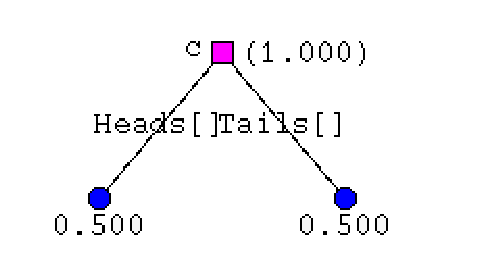
\includegraphics[scale=.6]{images/headOrTails.eps}
}
\caption{\lqpl{} program to do a coin flip}\label{fig:defsec:coin}
\end{figure}

In the function \inlqpl{cflip},  a \qbit{} is prepared by initializing it
to \ket{0} and applying the \Had{} transform. This creates a \qbit{} 
whose density matrix is {\begin{singlespace}$\begin{pmatrix}.5&.5\\ 
.5&.5\end{pmatrix}$\end{singlespace}}. When
 this \qbit{} is measured, it has a $50\%$ chance of being $0$ and 
an equal chance of being $1$. 

In the branches of the measure,  different values are assigned to the 
return variable $c$. Each of these assignments happens with a probability of
$50\%$. Once the measure statement is completed, the variable \inlqpl{c}
will be \inlqpl{Heads} and \inlqpl{Tails} each with a probability of $50\%$.
In the quantum stack machine this is represented as in 
sub-figure b of \vref{fig:defsec:coin}.


This illustrates the largest difference between quantum and classical 
processing of choices. In classical programming languages, a choice such
as a case type statement 
\emph{will only execute the code on one of the branches of the case}. 
In \lqpl{}, \emph{every} branch may be executed.


%\begin{wrapfigure}{l}{3in}
\begin{figure}[htbp]
\centering
\subfloat[Balanced creation]{
\begin{singlespace}
\lstinputlisting[style=linqpl]{examplecode/dataCreationExample1.qpl}
\end{singlespace}}
\qquad
\subfloat[Unbalanced creation]{
\begin{singlespace}
\lstinputlisting[style=linqpl]{examplecode/dataCreationUnbalanced.qpl}
\end{singlespace}}
\caption{\lqpl{} programs contrasting creation}
\label{fig:defsec:balancedcreation}
\end{figure}

When writing the dependent blocks of \inlqpl{measure}
 (and \inlqpl{case} in \vref{subsec:casestatements}) 
 variable creation must be
the same in each dependent list of statements.
 The compiler will give you a semantic
warning if a variable is created in one branch and not another.

For example, consider \vref{fig:defsec:balancedcreation}. In the left 
hand program on the 
\inlqpl{measure} starting at line \ref{line:measure1}, each branch creates a 
variable named '\inlqpl{i}'. This is legal and from line \ref{line:iexists}
forward,  '\inlqpl{i}' will be available.

On the other hand, the measure in the right hand program  starting in line 
\ref{line:measure2} assigns to the variable  '\inlqpl{c}' in
the \ket{0} branch and  '\inlqpl{d}' in the \ket{1} branch. At line
\ref{line:neitherdorc}, neither variable will be available. The compiler
will give the warnings:
\begin{quote}
\footnotesize
\terminalio{Warning: Unbalanced creation, discarding c of type INT}\\
\terminalio{Warning: Unbalanced creation, discarding d of type INT}
\end{quote}

\paragraph{Syntax of the \inlqpl{measure} statement.} This statement
starts with the word \emph{measure}, 
followed by a variable name, which must be of type \inlqpl{Qbit}. 
Next, the keyword \emph{of} signals the start of the two case selections.
 The case selection starts with either \ket{0} or \ket{1}, followed by
$=>$ and the block of dependent statements.

Note that \emph{both} case selections for a \qbit{} must be present. However,
it is permissible to not have any statements in a block.

\subsection{Case statement}\label{subsec:casestatements}
The \inlqpl{case} statement is used with any variable of a declared
datatype. 
\begin{figure}[htbp]
\begin{singlespace}
\lstinputlisting[style=linqpl]{examplecode/reverse.qpl}
\end{singlespace}
\caption[Reverse program to demonstrate \inlqpl{case}]{\lqpl{} program demonstrating \inlqpl{case}, a function to reverse a list.}
\label{fig:defsec:reverse}
\end{figure}  


In \vref{fig:defsec:reverse}, the program declares the
 \inlqpl{List} data type, which is parametrized by one
type variable and has two constructors: \inlqpl{Nil} which has no
arguments and \inlqpl{Cons} which takes two arguments of types
\inlqpl{a} and \inlqpl{List a} respectively.

The function \inlqpl{reverse} takes a list 
as an input argument and returns a single list, which is the original 
list in reverse order. Because of the linearity of the language
the original input list is not in scope at the end of the function.
The function \inlqpl{reverse} delegates to the function \inlqpl{rev'}
which uses an accumulator to hold the list as it is reversed.

The case statement begins on line \ref{line:rev:caserev}. For
\inlqpl{Nil}, it assigns the accumulator to the return list. For
\inlqpl{Cons}, it first adds the current element to the
front of the accumulator list, then it uses a recursive call
to reverse the tail of the original list with the new accumulator.


\begin{figure}[htbp]
\begin{singlespace}
\lstinputlisting[style=linqpl]{examplecode/treeMaxDepth.qpl}
\end{singlespace}
\caption[Tree depth program to demonstrate \inlqpl{case}]{\lqpl{} program demonstrating \inlqpl{case}, a function to compute the max tree depth.}
\label{fig:defsec:treemaxdepth}
\end{figure}

Considering the example in \vref{fig:defsec:treemaxdepth}. \inlqpl{TTree}
is a parametrized data type which depends on 
the type variable \inlqpl{a}. It
 has three constructors: \inlqpl{Tip} which takes no arguments;
\inlqpl{Br} which takes three arguments of types \inlqpl{TTree a, a} and
\inlqpl{TTree a}; and \inlqpl{Node} which takes one argument of type
\inlqpl{a}.

In \inlqpl{treeMaxDepth}, the case statement on line
\ref{line:flattenTree:casedepth} illustrates a ``don't care'' pattern for
both the \inlqpl{Node} and \inlqpl{Br} constructors. This function
 returns the maximum depth of the \inlqpl{TTree} and actually
discards  the actual data elements stored at nodes.



\paragraph{Syntax of the \inlqpl{case} statement.} This statement
starts with the word \emph{case}, 
followed by a variable   of some declared type.
Next, the keyword \emph{of} signals the start of the case selections.
The number of constructors in a type determine how many 
case selections the statement has. There is one selection 
for each constructor.
Each case selection consists of  a \emph{constructor pattern}, a
'$=>$' and dependent statements. 

Constructor patterns 
are the constructor followed by a parenthesized list of 
variables and / or \emph{don't care} symbols, '\_'.  Non-parametrized 
constructors appear without a list of variable names. The 
don't care symbol causes data to be discarded.

\subsection{Use and classical assignment statements}\label{subsec:usestatements}

The \inlqpl{use} statement is used with any variable of type \inlqpl{Int}
or \inlqpl{Bool}. 
This statement  has a single 
set of dependent statements. These may 
either be explicitly attached to the \inlqpl{use} statement or implicit.
Implicit dependent statements are all the statements following
the \inlqpl{use} until the end of the current block. 

Classical assignment is grouped here as it is syntactic sugar for a
\inlqpl{use} with implicit statements. This is illustrated in 
\ref{fig:useequalsassignment}.

%\begin{wrapfigure}{l}{2.75in}
\begin{figure}[htbp]
\begin{singlespace}
\begin{center}
\begin{tabular}{lcl}
$\vdots$ & & $\vdots$ \\
\begin{lstlisting}
i := exp;
s1;
\end{lstlisting} &
$\equiv$ &
\begin{lstlisting}
i = exp;
use i;
s1;
\end{lstlisting} \\
$\vdots$ & & $\vdots$
\end{tabular}
\end{center}
\end{singlespace}
\caption{Syntactic sugar for \inlqpl{use} / classical assignment}
\label{fig:useequalsassignment}
\end{figure}

The three types of classical use are semantically equivalent, but
do have different syntaxes as illustrated in \vref{fig:defsec:usestatements}.

\begin{figure}[htbp]
\centering
\subfloat[Explicit dependence]{
\begin{singlespace}
\lstinputlisting[style=linqpl]{examplecode/treeMaxDepth.explicit.frag.qpl}
\end{singlespace}}
\qquad
\subfloat[Implicit dependence]{
\begin{singlespace}
\lstinputlisting[style=linqpl]{examplecode/treeMaxDepth.frag.qpl}
\end{singlespace}}
\qquad
\subfloat[Classical assign]{
\begin{singlespace}
\lstinputlisting[style=linqpl]{examplecode/treeMaxDepth.cassign.frag.qpl}
\end{singlespace}}
\caption{Fragments of \lqpl{} programs contrasting \inlqpl{use} syntax}
\label{fig:defsec:usestatements}
\end{figure}

In sub-figure (a) of \ref{fig:defsec:usestatements}, the \inlqpl{use}
statement starts on line \ref{line:tmdfragexplicit:use}. The next two
statements are explicitly in its scope, which ends at line 
\ref{line:tmdfragexplicit:scopend}.  In sub-figure (b) of the same figure,
the \inlqpl{use} at line \ref{line:tmdfrag:use} is implicit. Its scope
extends to line \ref{line:tmdfrag:scopend}. Finally, in sub-figure(c),
the same effect is achieved with two classical assignments at 
lines \ref{line:tmdfragcas:assignj} and \ref{line:tmdfragcas:assignk}.
The scope of these assignments extend to line \ref{line:tmdfragcas:scopend}.


Unlike data types and \inlqpl{Qbit}s, which have a maximum number of 
sub-stacks, an \inlqpl{Int} has the potential to have 
 an unbounded number of values and therefore sub-stacks. 
The dependent statements of
 the \inlqpl{use} statement are executed for \emph{each} 
of these values.

To execute different pieces of code depending on the value, \lqpl{}
provides the \inlqpl{if} - \inlqpl{else} statement as discussed in
\vref{subsec:classicalcontrolstatements}.

\paragraph{Syntax of the \inlqpl{use} statement.} This statement starts with 
the word \inlqpl{use},
 followed by a list of variable names, which must be  of
type \inlqpl{Int} or \inlqpl{Bool}. If there is an 
explicit dependent block for the statement, it is given by the
keyword \inlqpl{in} followed by the dependent block.

When the \inlqpl{use} statement is \emph{not} followed by a dependent block, 
the rest of the statements in the enclosing block are considered in
the scope of the \inlqpl{use}.

Classical assign syntax is a variable name, followed by the 
symbol ':=' followed by an expression. The expression must have
type \inlqpl{Int} or \inlqpl{Bool}. 

\subsection{Function calls}\label{subsec:functioncalls}
Function calls include calling functions defined in  programs and
the predefined transforms. The list of predefined transforms valid
in a \lqpl{} program are given in \vref{tab:lqpltransforms}.
%TODO - Dr. C regarding transforms
% - reduce primitives, show how to get rest
% - Explain interdependence
% - reexamine formula for Rot, possibly use R(n,t) (t  an int), = 1 &0\\0&e^{-i t \pi / 2^{n-1}}
% - Remove RhoZ, Phase, T (Rot...) and Swap (=, =)
\begin{table}
\centerline{
\begin{tabular}{|l|l|c|}
\hline
\textbf{\lqpl{}}& \textbf{A.K.A.} & \textbf{Matrix} \\
\hline 
& & \\
\inlqpl{Not} & $X$, Pauli-X, $\rho_X$  & $ 
\begin{bmatrix}
0&1\\
1&0
\end{bmatrix}$ \\ & & \\\hline
 & &  \\
\inlqpl{RhoY} & $Y$, Pauli-Y, $\rho_Y$ &
$ 
\begin{bmatrix}
0&-i\\
i&0
\end{bmatrix}$ \\ & & \\\hline
 & &  \\
\inlqpl{RhoZ (=Rot(0))} & $Z$, Pauli-Z, $\rho_Z$ &
$ 
\begin{bmatrix}
1&0\\
0&-1
\end{bmatrix}$ \\ & & \\\hline
 & &  \\
\inlqpl{Had} & Had, $H$ &
$ 
\frac{1}{\sqrt{2}}\begin{bmatrix}
1&1\\
1&-1
\end{bmatrix}$ \\ & & \\\hline
& & \\
\inlqpl{Swap} & Swap &
$ 
\begin{bmatrix}
1&0&0&0\\
0&0&1&0\\
0&1&0&0\\
0&0&0&1
\end{bmatrix}$ \\ & & \\\hline
& & \\
\inlqpl{Phase (=Rot(2))} & $S$, Phase $\sqrt{Z}$ &
$
\begin{bmatrix}
1&0\\
0&i
\end{bmatrix}$ \\ & & \\\hline
& & \\
\inlqpl{T(=Rot(3))} & $T$, $\frac{\pi}{8}$, $\sqrt{S}$ &
$
\begin{bmatrix}
1&0\\
0&e^{i\pi/4}
\end{bmatrix}$ \\ & & \\\hline
& & \\
\inlqpl{Rot(n)} & $R_n$, Rotation &
$
\begin{bmatrix}
1&0\\
0&e^{i\pi/2^{n-1}}
\end{bmatrix}$ \\ & & \\\hline
\end{tabular}
} 
\caption{\lqpl{} transforms}\label{tab:lqpltransforms}
\end{table}

In addition to the predefined transforms, \lqpl{}
 allows you to prefix any of the 
predefined transformations with the 
string \inlqpl{Inv-} to get the inverse transformation. Controlled versions 
of all of these are available by using the quantum control construction
as defined in \vref{subsec:quantumcontrol}.
 For example,  the \inlqpl{Toffoli3} gate
as shown in \vref{tab:qgatesAndRep} is simply a  controlled-controlled-Not 
transformation.

The signatures of transforms are dependent upon the size of the 
associated matrix. A $2\times 2$ matrix gives rise to the signature
\inlqpl{(q:Qbit ; q:Qbit)}. In general, a $2^n \times 2^n$ matrix
will require $n$ \qbit{}s in and out. The parametrized transforms such
as \inlqpl{Rot} will  require one or more integers as input.

\subsubsection{Syntax of function calls}\label{subsubsec:syntaxfunction}
There are three different calling syntaxes for functions:
\begin{enumerate}
\item{} \emph{Functional} --- $(y_1,\dots,y_m) = f(n_1,\dots,n_k\, |\, x_1,\dots,x_j).$
\item{} \emph{Procedural} ---  $f(n_1,\dots,n_k\, |\, x_1,\dots,x_j\, ;\, y_1,\dots,y_m).$
\item{} \emph{Transformational} --- $f(n_1,\dots,n_k )\ z_1\ z_2\ \dots\ z_j.$
\end{enumerate}


\paragraph{Functions with classical and quantum inputs.}
These functions  may be called\footnote{A function
call with a  single unparenthesized variable appears on the
left hand side of the equals
 are
 actually assignment statements. The  right hand side of the assignment 
is a function expression.
See \vref{subsec:expressioncalls}} in each of the
three ways.
\begin{lstlisting}
      f ::(c1:Int,c2:Int, c3:Int | q1:Qbit, i1:Int ; a:Qbit, b:Int)
      = { ... }
      ...
         (a,b) = f(c1,c2,c3 | q1,i2);
         f(c1,c2,c3 | q1,i2; a,b);
         f(c1,c2,c3) q i;
\end{lstlisting}

When a function is called in the transformational syntax, as on the last 
line of the above code, the arguments (\inlqpl{q i} in the example) are 
both passed into
the function as arguments and used as return variables. 
The arguments in the parenthesis ( \inlqpl{c1,c2,c3} in our example),
\emph{must} be classical and a
 semantic error will result if a quantum variable is used.
If the number of in and out quantum arguments are not the same
or their types
do not match, this syntax is not available.


\paragraph{Functions which have no quantum input arguments.}
Functions which have only classical  inputs 
may be called in either the functional or procedural 
syntax. As there are no input quantum arguments, transformational
syntax is not allowed.

\begin{lstlisting}
      g :: (c1:Int, c2:Int | ; r:Int, d:Int) 
      = { ... }
      ...
        (a,b) = g(c1,c2 |);
        g(c1,c2 | ; a,b);
\end{lstlisting}


\paragraph{Functions which have no classical input arguments.}
Functions having only quantum  inputs may use
all three syntaxes. In this case, where the classical
variable list of arguments is empty, the ``|'' may 
be eliminated in procedural or functional calling, and the 
parenthesis may be eliminated in transformational calling.

\begin{lstlisting}
      h :: (q1:Int, q2:Int ; r:Int, d:Int) 
      = { ... }
      ...
        (a,b) = h(|c,d);
        (a,b) = h(c,d);
        h(|a,b ; c,d);
        h(a,b; c,d);
        h a b;
\end{lstlisting}



\paragraph{Linearity of function call arguments.}
Each input argument is no longer in scope after the function call. If 
the input is a simple identifier, the same identifier may be used in
the output list of the function. The transformational
syntax uses this technique to leave the variable names unchanged.

\paragraph{Syntactic forms of function and transform calls.}
In all three of the forms for function calling, the number and type
of input arguments must agree with the definition of the function.
Output identifiers must agree in number and their type is set according
to the definition of the functions output parameters. Output
variables are always quantum.

The  \emph{functional} syntax for function calling has three parts.
The first part is a parenthesized  list of variable names separated by 
commas.
The parenthesized list is then followed by an equals sign. The right hand side
 consists of the function name
followed by the  parenthesized  input arguments. The input arguments 
consists of two lists of arguments separated by '\inlqpl{|}'. The first
list consists of the classical arguments, the second of the quantum arguments.
Each argument must be a valid expression as defined 
in  \vref{sec:lqplexpressions}.
 If there are no classical arguments, the '\inlqpl{|}' is optional.


The  \emph{procedural} syntax for function calling starts with the
function name, followed by a parenthesized grouping of input and
output arguments.  As in the functional form, the list of classical input 
arguments are separated from the quantum ones by '\inlqpl{|}', which may
be eliminated when there are no classical arguments. The input arguments
are separated from the output arguments by '\inlqpl{;}'. 

The \emph{transformational} syntax starts with the
function name followed  by a parenthesized list of classical
expressions and then by a series of identifiers, separated by white space.
A requirement for using this syntax is that the
number and types of the input and output quantum arguments must be the same. 
The identifiers will be passed as input to the function and will be
returned by the function. The parenthesis for the list of classical
expressions may be eliminated when there are no classical parameters.


Function calls may also be expressions, which is discussed in
\vref{subsec:expressioncalls}.

\subsection{Blocks}\label{subsec:blocks}
Blocks are created by surrounding a list of statements with braces. A 
block may appear wherever a statement does.  All of the ``grouping''
types of statements require blocks rather than statements as their group.
See, for example, the discussion on \inlqpl{case} statements
in \vref{subsec:casestatements}.

\subsection{Quantum control}\label{subsec:quantumcontrol}

Quantum control provides a general way to create and use controlled unitary 
transforms in an \lqpl{} program. 
An example of quantum 
control is shown in the prepare and teleport functions in
 \vref{fig:defsec:stmts:demoofcontrol}.


\begin{figure*}[htbp]
\begin{singlespace}
\lstinputlisting[style=linqpl]{examplecode/teleport.qpl}
\end{singlespace}
\caption{\lqpl{} program demonstrating quantum control}
\label{fig:defsec:stmts:demoofcontrol}
\end{figure*}

\paragraph{Syntax of quantum control}
In \lqpl{} any statement, including block statements and 
procedure calls may be quantum controlled.
Semantically, this will  affect all transforms that occur within
the controlled statement, including
any of the transforms in a called function.
The  syntax is \emph{statement} 
followed by the symbols \emph{<=}, followed
by a list of identifiers.  These identifiers may 
be of any type, but are typically
either \qbit{}s or constructed data types with \qbit{} elements, such as a 
\inlqpl{List(Qbit)}.

The identifiers that are controlling a statement can not be used
in the statement. Controlling identifiers are exempt from
linearity constraints in that they remain in scope after the
quantum control construction.

The effect of the control is that all \qbit{}s in the 
control list, or contained in items
in that list are used to control all unitary 
transformations done in the controlled
statement.

\subsection{Divergence}\label{subsec:nontermination}
To force the execution  of a program  to diverge, you can use the
\inlqpl{zero} statement. This will set the probability of the values of
a program to 0, and is interpreted as non-termination.

\subsection{Discard}\label{subsec:discard}
In some algorithms, such as  in recursive functions when they process
the initial cases of constructed data,
the algorithm does not specify any action. In these cases, the programmer
may need to examine the requirements of linearity with respect to 
any passed in parameters. Often, these will need to be explicitly
discarded in base cases of such algorithms.
This is done via the discard statement.
An example may be seen in \vref{fig:inverserotate}.